%%%%%%%%%%%%%%%%%%%%%%%%%%%%%%%%%%%%%%%%%
% Beamer Presentation
% LaTeX Template
% Version 1.0 (10/11/12)
%
% This template has been downloaded from:
% http://www.LaTeXTemplates.com
%
% License:
% CC BY-NC-SA 3.0 (http://creativecommons.org/licenses/by-nc-sa/3.0/)
%
%%%%%%%%%%%%%%%%%%%%%%%%%%%%%%%%%%%%%%%%%

%----------------------------------------------------------------------------------------
%	PACKAGES AND THEMES
%----------------------------------------------------------------------------------------

\documentclass{beamer}

\mode<presentation> {

% The Beamer class comes with a number of default slide themes
% which change the colors and layouts of slides. Below this is a list
% of all the themes, uncomment each in turn to see what they look like.

%\usetheme{default}
%\usetheme{AnnArbor}
%\usetheme{Antibes}
%\usetheme{Bergen}
%\usetheme{Berkeley}
%\usetheme{Berlin}
%\usetheme{Boadilla}
%\usetheme{CambridgeUS}
%\usetheme{Copenhagen}
%\usetheme{Darmstadt}
%\usetheme{Dresden}
%\usetheme{Frankfurt}
%\usetheme{Goettingen}
%\usetheme{Hannover}
%\usetheme{Ilmenau}
%\usetheme{JuanLesPins}
%\usetheme{Luebeck}
\usetheme{Madrid}
%\usetheme{Malmoe}
%\usetheme{Marburg}
%\usetheme{Montpellier}
%\usetheme{PaloAlto}
%\usetheme{Pittsburgh}
%\usetheme{Rochester}
%\usetheme{Singapore}
%\usetheme{Szeged}
%\usetheme{Warsaw}

% As well as themes, the Beamer class has a number of color themes
% for any slide theme. Uncomment each of these in turn to see how it
% changes the colors of your current slide theme.

%\usecolortheme{albatross}
%\usecolortheme{beaver}
%\usecolortheme{beetle}
%\usecolortheme{crane}
%\usecolortheme{dolphin}
%\usecolortheme{dove}
%\usecolortheme{fly}
%\usecolortheme{lily}
%\usecolortheme{orchid}
%\usecolortheme{rose}
%\usecolortheme{seagull}
%\usecolortheme{seahorse}
%\usecolortheme{whale}
%\usecolortheme{wolverine}

%\setbeamertemplate{footline} % To remove the footer line in all slides uncomment this line
%\setbeamertemplate{footline}[page number] % To replace the footer line in all slides with a simple slide count uncomment this line

%\setbeamertemplate{navigation symbols}{} % To remove the navigation symbols from the bottom of all slides uncomment this line
}

\usepackage{graphicx} % Allows including images
\usepackage{booktabs} % Allows the use of \toprule, \midrule and \bottomrule in tables
\graphicspath{ {jpegs/} }

%----------------------------------------------------------------------------------------
%	TITLE PAGE
%----------------------------------------------------------------------------------------

\title[Forward shooting grid]{Forward shooting grid method \\ for arithmetic average options} % The short title appears at the bottom of every slide, the full title is only on the title page

\author{Mircea Simionica} % Your name
\institute[] % Your institution as it will appear on the bottom of every slide, may be shorthand to save space
{
\medskip
\textit{Applied Numerical Finance assignment} % Your email address
}
\date{December 3, 2015} % Date, can be changed to a custom date


\begin{document}

\begin{frame}[noframenumbering,plain]
\titlepage % Print the title page as the first slide
\end{frame}


\begin{frame}
\frametitle{Overview} % Table of contents slide, comment this block out to remove it
\tableofcontents % Throughout your presentation, if you choose to use \section{} and \subsection{} commands, these will automatically be printed on this slide as an overview of your presentation
\end{frame}

%----------------------------------------------------------------------------------------
%	PRESENTATION SLIDES
%----------------------------------------------------------------------------------------
\section{Average options} % Sections can be created in order to organize your presentation into discrete blocks, all sections and subsections are automatically printed in the table of contents as an overview of the talk
%------------------------------------------------
\begin{frame}
\frametitle{Average options}
\begin{itemize}
\item Asian options provide a cost-efficient way of hedging
\item More attractive to some investors because less expensive and less volatile
\item Payoff:
\begin{align*}
\text{Average call (fixed strike)} \rightarrow X(T) &= (S_{average}-K)^+ \\
\text{Asian call (floating strike)} \rightarrow X(T) &= (S_T - S_{average})^+
\end{align*}
\item Standard form of averaging is arithmetic $\Rightarrow$ valuation is not trivial
\begin{itemize}
\item Arithmetic average has no simple analytic shape
\item In classical binomial model the number of averages \\ grows exponentially with the size of the tree
\end{itemize}
\end{itemize}

\end{frame}
%------------------------------------------------
\section{Forward shooting grid for arithmetic average options} % Sections can be created in order to organize your presentation into discrete blocks, all sections and subsections are automatically printed in the table of contents as an overview of the talk
%------------------------------------------------
\begin{frame}
\frametitle{Forward shooting grid for arithmetic average options}
\begin{columns}[c] % The "c" option specifies centered vertical alignment while the "t" option is used for top vertical alignment

\column{.30\textwidth} % Left column and width
\textbf{Steps}
\begin{enumerate}
\item Build tree for S
\end{enumerate}

\column{.60\textwidth} % Right column and width
\begin{figure}
	\includegraphics[scale=0.4]{lattice2.png}
\end{figure}

\end{columns}
\end{frame}

\begin{frame}[noframenumbering]
\frametitle{Forward shooting grid for arithmetic average options}
\begin{columns}[c] % The "c" option specifies centered vertical alignment while the "t" option is used for top vertical alignment

\column{.45\textwidth} % Left column and width
\textbf{Steps}
\begin{enumerate}
\item Build tree for S
\item Shoot averages
\end{enumerate}

\column{.5\textwidth} % Right column and width
\begin{figure}
	
\includegraphics[scale=0.1]{forward}
\end{figure}
\begin{figure}
	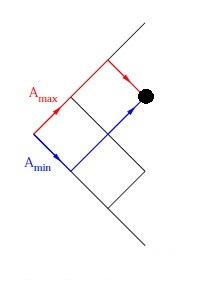
\includegraphics[scale=0.5]{average_path}
\end{figure}

\end{columns}
\end{frame}

\begin{frame}[noframenumbering]
\frametitle{Forward shooting grid for arithmetic average options}
\begin{columns}[c] % The "c" option specifies centered vertical alignment while the "t" option is used for top vertical alignment

\column{.45\textwidth} % Left column and width
\textbf{Steps}
\begin{enumerate}
\item Build tree for S
\item Shoot averages
\item Backward recursion
\end{enumerate}

\column{.5\textwidth} % Right column and width
\begin{figure}
	
\includegraphics[scale=0.1]{backward}
\end{figure}
\begin{figure}
	
\includegraphics[scale=0.4]{question_mark}
\end{figure}

\end{columns}
\end{frame}

%------------------------------------------------

\section{Numerical and financial remarks}

\begin{frame}
\frametitle{Numerical and financial remarks}
\begin{columns}[t] % The "c" option specifies centered vertical alignment while the "t" option is used for top vertical alignment

\column{.45\textwidth} % Left column and width
\textbf{Numerical POV}
\begin{itemize}
\item How to space values in the average vector
\item Interpolation type
\item Number of time steps and dimension of the average vector
\end{itemize}

\column{.45\textwidth} % Left column and width
\textbf{Financial POV}
\begin{itemize}
\item What about discrete sampling?
\item Greeks
\end{itemize}

\end{columns}
\end{frame}
%------------------------------------------------
\section{Programming remarks}

\begin{frame}
\frametitle{Programming remarks}

\begin{block}{Main issue}
Data structure that will store the lattices.
\end{block}
\vspace{10mm}
\begin{columns}[c] % The "c" option specifies centered vertical alignment while the "t" option is used for top vertical alignment

\column{.60\textwidth} % Left column and width
\textbf{Bad version}
\begin{enumerate}
\item Lattice for S held in a matrix of doubles
\item Averages and option prices held in a field (matrix of vectors)
\end{enumerate}
\vspace{5mm}
$\Rightarrow$ perfect recipe for memory bottlenecks

\column{.30\textwidth} % Left column and width
\begin{figure}
	
\includegraphics[scale=0.8]{no}
\end{figure}

\end{columns}
\end{frame}

%------------------------------------------------
\begin{frame}
\frametitle{Programming remarks}

\begin{block}{Main issue}
Data structure that will store the lattices.
\end{block}
\vspace{10mm}

\begin{columns}[b] % The "c" option specifies centered vertical alignment while the "t" option is used for top vertical alignment

\column{.20\textwidth} % Left column and width
\begin{figure}
	
\includegraphics[scale=0.13]{yes}
\end{figure}

\column{.72\textwidth} % Left column and width
\textbf{A better way to do it}
\begin{enumerate}
\item Lattice for S held in a sparse matrix
\item Averages held in a C++ vector$<\text{data type}>$ (STL dynamic container)
\item Option prices just a vector of vectors (for every timestep we only need data from the step ahead)
\end{enumerate}

\end{columns}
\end{frame}


%------------------------------------------------
\section{Numerical results}

\begin{frame}
\frametitle{Some numerical results}
\begin{center}
Arithmetic average option from Hull (page 613)\\
$S_0=50, K = 50, r = 0.10, \sigma = 0.40, T = 1$ \\
Analyitic approximation with continuous averaging: $5.62$
\end{center}

\begin{table}
\begin{tabular}{c c c c}
\toprule
\textbf{\# time steps} & \textbf{\# averages} & \textbf{Option price} & \textbf{Time (seconds)}\\
\midrule
200	&	100	&	6.16638	&	0.796763	\\
200	&	200	&	5.70347	&	1.98051	\\
200	&	400	&	5.59344	&	5.96032	\\
200	&	600	&	5.57341	&	12.2608	\\
200	&	800	&	5.56831	&	20.5464	\\
200	&	1000	&	5.56491	&	31.1804	\\
200	&	1500	&	5.56191	&	67.1026	\\
200	&	2000	&	5.56086	&	116.902	\\
200	&	2500	&	5.56038	&	179.459	\\
200	&	3000	&	5.56011	&	259.534	\\
\bottomrule
\end{tabular}
\end{table}
\end{frame}

%------------------------------------------------

\begin{frame}
\vspace*{-1cm}
\frametitle{Some convergence results}
\begin{figure}[t]
	\includegraphics[scale=0.24]{convergence}
\end{figure}
\end{frame}

%------------------------------------------------

\begin{frame}
\frametitle{The end}
\begin{figure}
	\includegraphics[scale=0.35]{end_3}
\end{figure}
\end{frame}

%------------------------------------------------

\end{document} 